\documentclass[12pt, a4paper, twoside]{article}

%% Preamble
\usepackage{umatfgenglish}
\usepackage{blindtext}
\graphicspath{ {./images/} }

\begin{document}

% Crear mi propia portada en un futuro
%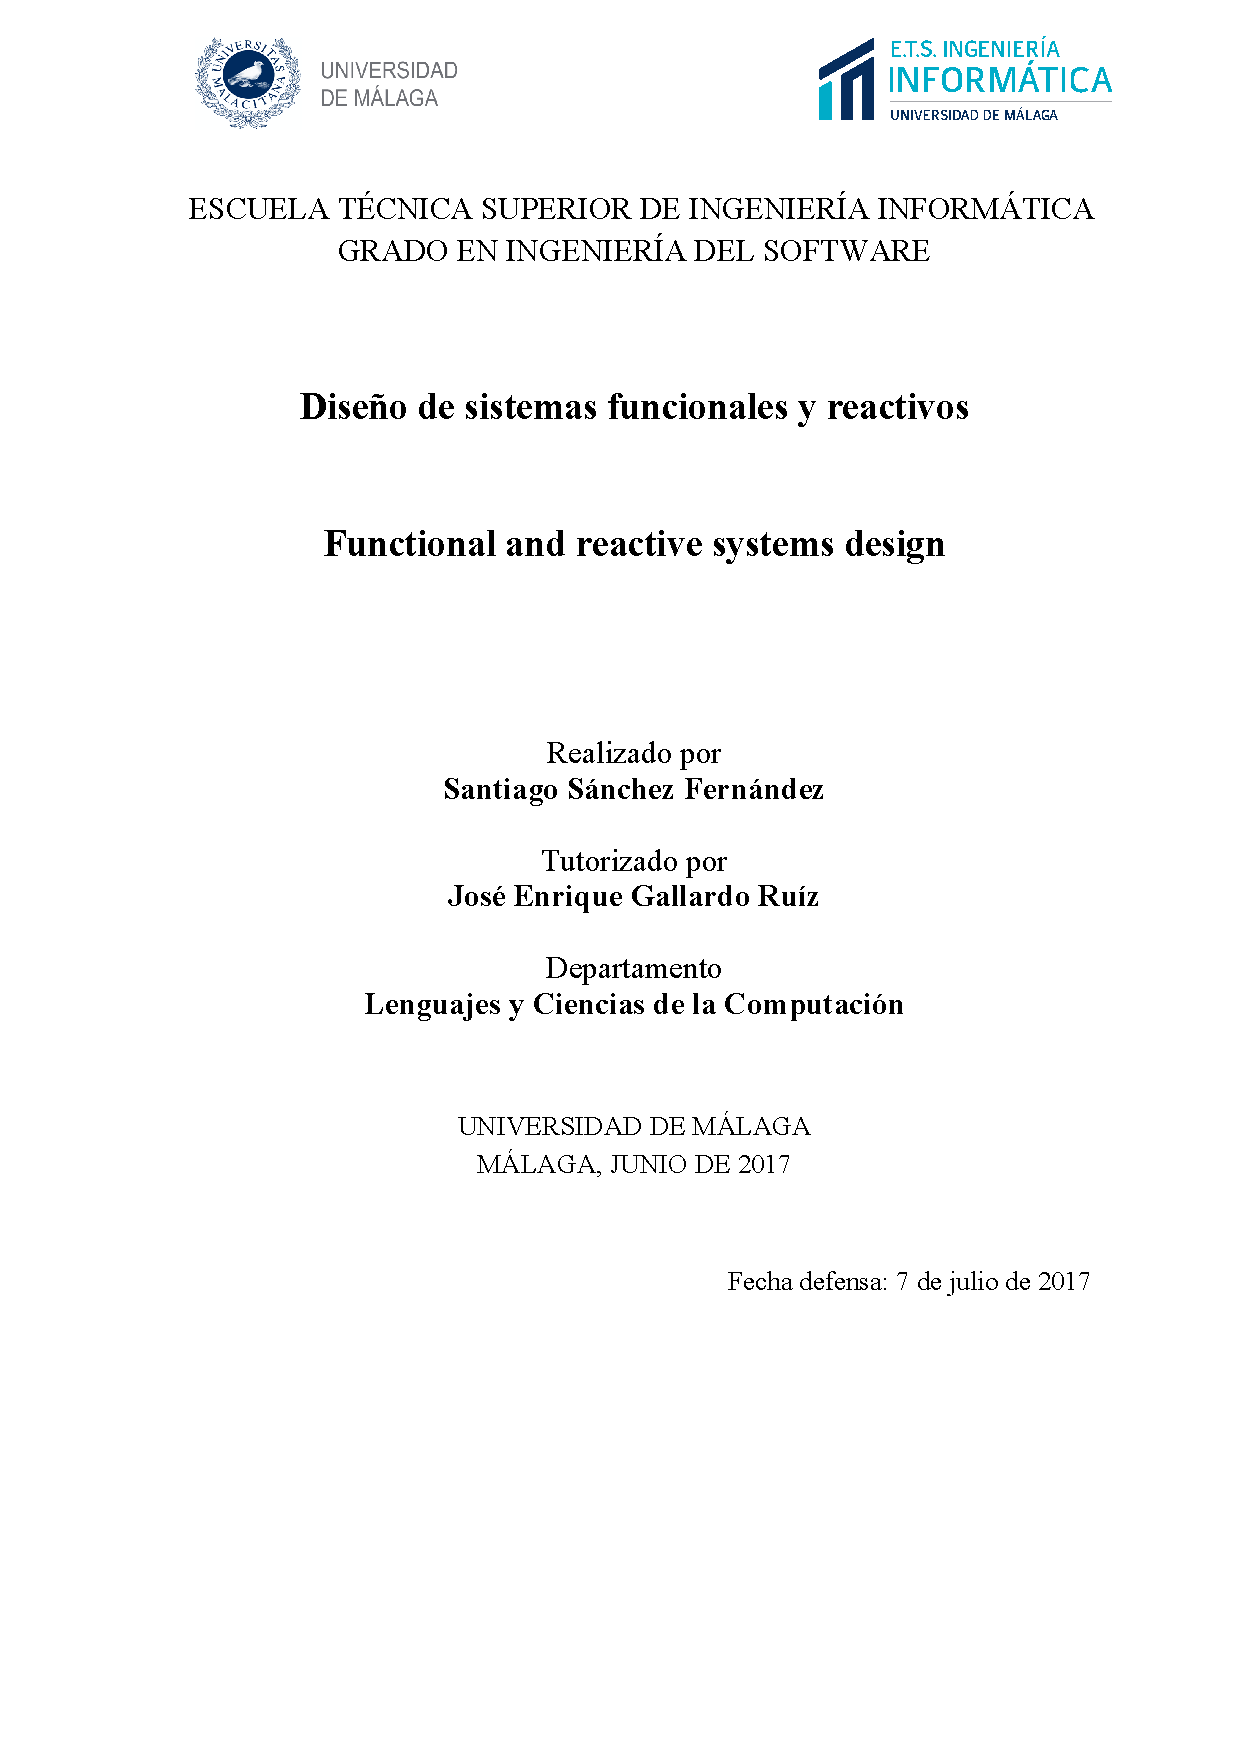
\includepdf[noautoscale=true, width=\paperwidth]{title.pdf}

\newpage

%% Abstract
\begin{abstract}
    Resumen corto del trabajo y palabras clave.
	\bfseries{\large{Keywords:}}
\end{abstract}

\tableofcontents

%% Sections
\section{Introducción}

\subsection{Motivation}
    Comenzar a desarrollar algo de esta embergadura es abrumador en las primeras instancias, sobre todo,
    si no se tiene experiencia previa. Enfrentarse a un trabajo de fin de carrera, recopilar todos los conocimientos
    adquiridos a lo largo de los años y aplicarlos en un proyecto real, es una tarea titánica. Por ello, es importante
    que sientas pasión y curiosidad por el tema elegido.
    \\
    El desarrollo de algoritmos metaheurísticos es un campo fascinante que combina la teoría de la computación,
    la optimización y la inteligencia artificial, y que tiene aplicaciones en una amplia variedad de áreas, desde la logística
    hasta la biología computacional, demostrando su versatilidad y utilidad en entornos reales. 
    
    \begin{figure}[h]
      \centering
        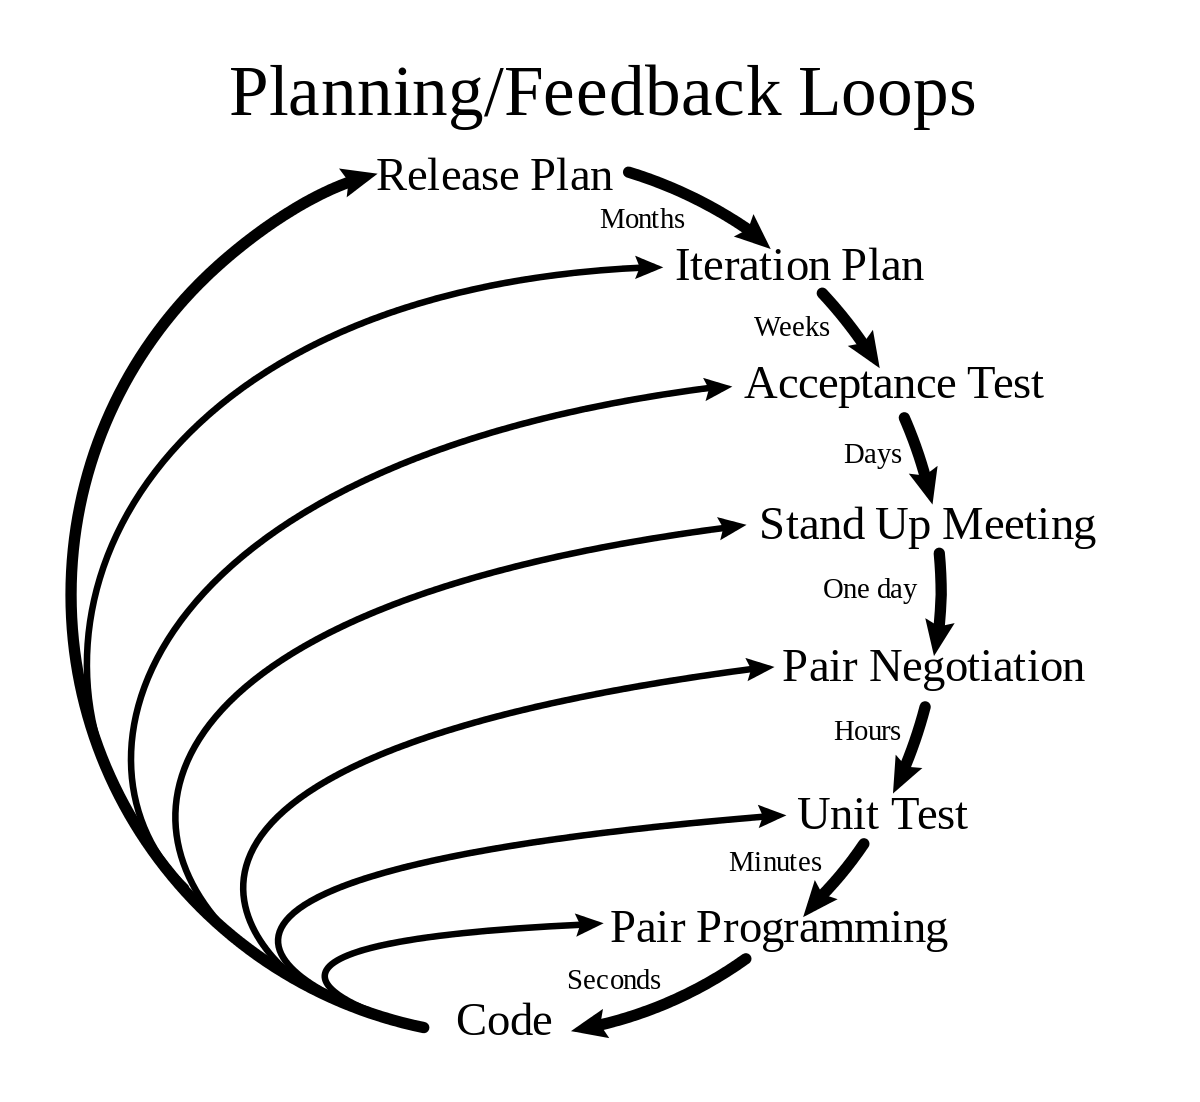
\includegraphics[width=0.5\textwidth]{xp}
      \caption{A diagram showing the iterations of extreme programming.}
    \end{figure}
    
    \blindtext[4]

\subsection{Objetivos}

\subsection{Tecnologías a utilizar}

\section{Metodología de trabajo \\}
    \blindmathpaper

\section{Desarrollo}

\section{Conclusiones y líneas futuras}

%% Bibliography
\begin{thebibliography}{9}
    \bibitem{latexcompanion} 
    Michel Goossens, Frank Mittelbach, and Alexander Samarin. 
    \textit{The \LaTeX\ Companion}. 
    Addison-Wesley, Reading, Massachusetts, 1993.
    
    \bibitem{einstein} 
    Albert Einstein. 
    \textit{Zur Elektrodynamik bewegter K{\"o}rper}. (German) 
    [\textit{On the electrodynamics of moving bodies}]. 
    Annalen der Physik, 322(10):891–921, 1905.
\end{thebibliography}

\newpage

%% Apendices
\begin{umaappendices}
\section{Installation \\ Manual}
    
    \textbf{\large{Requirements:}}
    
    \blindtext

\end{umaappendices}

\end{document}
